%ChapterVI.tex
\section{数字信号的频带传输}\label{chapter:VI}
\HyperBack{chapter:VI}
\subsection{引言}
    数字基带信号通过正弦型载波调制成为带通型频带信号。
    该数字调制的基本原理是用数字基带信号去控制正弦型载波的某\emph{参量}。
    且带通型数字调制有二进制和$M$进制($M>2$)之分。
    如:
    \begin{enumerate}[itemsep=0pt,parsep=0em,label=\color{bupt}\arabic*、,labelsep=0pt,leftmargin=4em]
        \item 控制载波的幅度,称为振幅键控(ASK);
        \item 控制载波的频率,称为频率键控(FSK);
        \item 控制载波的相位,称为相位键控(PSK);
        \item 联合控制载波的幅度和相位两个参量,称为正交幅度调制(QAM)。
    \end{enumerate}

    数字调制还以线性调制和非线性调制分类。
    线性调制要求从数字序列映射为相继的信号波形符合叠加原理。
    反之则为非线性调制。

    数字调制还以无记忆调制和有记忆调制来分类。
    若映射的波形与前面一个或多个码元有关,则称为有记忆,
    反之则为无记忆。

\subsection{二进制数字信号的正弦型载波调制}  
    \subsubsection{二进制启闭键控(OOK/2ASK)}
    OOK(On-Off Keying),即用二进制数字基带信号控制正弦载波的幅度。
    表达式为:
    \begin{equation}
        \begin{split}
            s_{\text{OOK}}(t)   &=A\left[\sum_{n=-\infty}^{\infty}a_ng_T(t-nT_b)\right]\cos(2\pi f_c t)\hspace{2em},a_n\in\{0,1\}\\
                                &=\begin{cases}
                                    A\cos(2\pi f_ct)\phantom{0}\hspace{3em}\text{“传号”}\\
                                    0\phantom{A\cos(2\pi f_ct)}\hspace{3em}\text{“空号”}
                                \end{cases}\hspace{1.5em},0\leq t\leq T_b
        \end{split}
    \end{equation}

    由表达式可见,这种信号有两种产生方式,
    一是利用类似于第五章成型滤波器的方案(即书上\emph{图6.2.1});
    另一种则是使用数字信号通过开关电路控制余弦信号的有无,
    这时候,也可以按照调制系数$a=1$的\hyperref[subsubsec:AM]{AM调制}或者
    基带信号为单极性不归零码的\hyperref[subsubsec:DSB-SCAM]{DSB调制}理解。

    可以根据\eqaref{eq:idd-PAM-Pf}得到OOK调制信号的功率谱密度
    \begin{equation}
        \begin{split}
            P_s(f)&=\frac{A^2}{4}[P_b(f-f_c)+P_b(f+f_c)]\\
            P_b(f)&=\sigma_a^2T_b\text{sinc}^2(fT_b)+m_a^2\delta(f)
        \end{split}
    \end{equation}
    其主瓣带宽为两倍基带带宽,即$2R_s$。

    OOK信号可以类比特殊的PAM数字调制,也可以类比AM模拟调制。
    所以可以有三类解调方式:
    \vspace{-2ex}

    \begin{enumerate}[itemsep=0pt,parsep=0em,label=\color{bupt}\arabic*、,labelsep=0pt,leftmargin=4em]
        \item 匹配滤波器
        \item LPF相干解调
        \item 非相干解调(包络检波)
    \end{enumerate}

    \paragraph{匹配滤波器}\mbox{}

    在$f_c\gg R_s$的时候,认为一个码元对应的波形是整数个载波周期\footnote{这样对于理论分析比较方便,实际上如果不是整数个周期,则稍微复杂,但在近似下得到的结果类似。}。
    匹配滤波器输出为
    \begin{figure}[H]
        \centering
        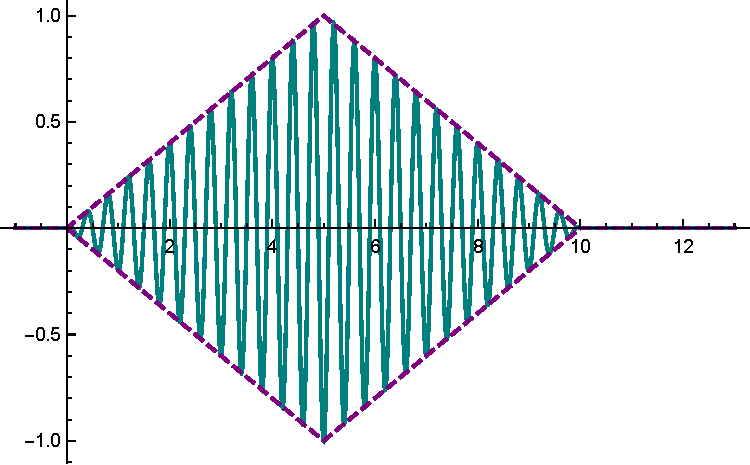
\includegraphics[scale=0.8]{body/image/book626.pdf}
        \caption{匹配滤波器输出}
    \end{figure}
    \emph{采样值为每一比特信号的能量$E_1=\dfrac{A^2T_b}{2}$}

    可见该方法对于定时要求比较高,若稍偏离最佳采样时刻,则会导致有用信号大幅减少。

    因为OOK可以看作PAM单极性不归零码在$g_T(t)=A\cos(2\pi f_c t)$时候的特例,
    故对于抗噪声性能可以使用类似的分析。这里直接引用结论:在平均比特能量为$E_b=\dfrac{E_1}{2}$时,误比特率
    \begin{equation}
        P_b=\frac{1}{2}\text{erfc}\left(\sqrt{\frac{E_1}{4N_0}}\right)=\frac{1}{2}\text{erfc}\left(\sqrt{\frac{E_b}{2N_0}}\right)
    \end{equation}

    \paragraph{LPF相干解调}\mbox{}

    把调制信号视作DSB信号,先与相干载波相乘得到混有高频成分的基带信号,
    再通过基带\footnote{顺便滤掉了高频成分}的匹配滤波器(相关器)输出,
    然后在最佳采样时刻采样。因为相乘的滤波的过程等价于频带的匹配滤波器,
    所以其性能也与上一种方式相同。
    
    但这种方式也会出现与\hyperref[subsubsec:DSB-SCAM]{DSB调制}一样的问题,
    及当解调用的正弦波和接收信号的载波同频但不同相的时候,则会出现采样值受到相位差的影响。
    
    在上两种方法中,如果需要考虑到限带系统ISI传输,也可以将发送滤波器设计成升余弦的形式,
    仍然不改变信噪比公式的形式。

    \paragraph{非相干解调}\mbox{}
    
    为了解决上一种方式中采样值受相位差的影响较为严重的问题,
    在通过带通滤波器(频带的匹配滤波器)后,再经过包络检波器。
    使用包络进行检测和判决。

    当发送“传号”的时候,接收信号为余弦信号叠加AWGN,
    其复包络服从\hyperref[eq:Rician-distribution]{莱斯分布};
    当发送“空号”的时候,接收到的信号只有AWGN,
    其复包络服从\hyperref[eq:Rayleigh]{瑞利分布}。

    在\emph{高信噪比}\footnote{看看\hyperref[subsubsec:AM]{AM调制},也是低信噪比不能工作。}
    的情况下,平均误比特率为
    
    \vspace{-2ex}
    \begin{equation}
        P_b\approx\frac{1}{2}e^{-\frac{E_b}{2N_0}}+\frac{1}{2}\cdot\frac{1}{2}\text{erfc}\left(\sqrt{\frac{E_b}{2N_0}}\right)\approx\frac{1}{2}e^{-\frac{E_b}{2N_0}}
    \end{equation}
    \vspace{-2ex}
    其性能逊于相干解调。

    \subsubsection{二进制频移键控(2FSK)}
    用二进制数字基带信号去控制正弦波载频的频率称为二进制频移键控(2FSK)。
    此时不妨用$f_1$与$f_2$($f_1>f_2$)分别对应"传号"和"空号"。
    2FSK可以按照相位连续和不连续分为两类。
    
    前者使用一个数字开关,通过不同的数字信号,把不同频率的载频振荡器接入线路。
    两个振荡器切换的时候,几乎不能\footnote{无内鬼,来点“实数轴几乎处处不为零”的测度论笑话}做到信号的相位连续。

    后者则使用类似于角度调制时使用的压控振荡器(VCO),中心频率为$f_c$,使用\emph{双极性归零码}来控制。
    不妨令$f_c=\dfrac{f_1+f_2}{2}$,则有最大频偏$\Delta f=\dfrac{f_1-f_2}{2}$。
    那么发送信号
    \vspace{-2ex}

    \begin{equation}
        s_{\text{FSK}}(t)=
        \begin{cases}
              A\cos[2\pi(f_c+\Delta f)t]\hspace{1em}\text{“传号”}\\
              A\cos[2\pi(f_c-\Delta f)t]\hspace{1em}\text{“空号”} 
        \end{cases}\hspace{2em}0\ll t\ll T_b
    \end{equation}

    为方便后文分析,这里先计算空号与传号之间的\hyperref[eq:Correlation-coefficient]{归一化相关系数}:
    \begin{equation}\label{eq:rhoof2fsk}
        \rho_{12}=\frac{<s_1(t),s_2(t)>}{\sqrt{E_{s_1}E_{s_2}}}=\text{sinc}(4\Delta fT_b)
    \end{equation}

    可见两个信号正交的条件为:$2\Delta f=n\cdot\dfrac{R_b}{2},n\in N_+$ 或$2\Delta f\gg R_b$\footnote{注意不同相的时候分析结果也会有所不同。}。

    接下来讨论2FSK信号的\emph{功率谱密度}。

    分析可知,相位不连续2FSK的功率谱旁瓣以$\dfrac{1}{f^2}$的速度衰减,
    而相位连续的2FSK的功率谱旁瓣以$\dfrac{1}{f^4}$的速度衰减。
    所以我们主要考虑\emph{相位连续}的2FSK信号。

    如果把2FSK信号视作两个“互补”的不同频率但\emph{正交}的OOK信号,
    其功率谱的形状则是两个OOK的功率谱直接叠加,
    两个功率谱的最大值相距为$f_1-f_2=2\Delta f$。各自由向左右延伸一个基带带宽$W$,
    故总的带宽为$B_\text{2FSK}=2\Delta f+2W$。
    \begin{figure}[H]
        \centering
        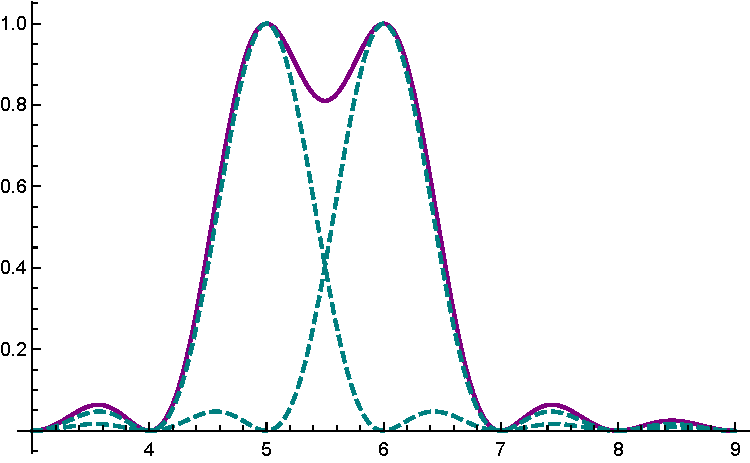
\includegraphics[scale=0.8]{body/image/2FSKPSD.pdf}
        \caption{2FSK信号的功率谱}
    \end{figure}
    带宽当然也可以类比FM调制,直接使用\hyperref[eq:Carson]{卡松公式},
    得到$B_\text{2FSK}=2\Delta f+2W$

    对于2FSK信号的解调也有相干解调与非相干解调的两种方式
    
    \paragraph{相干解调}\mbox{}

    假设使用分别匹配“传号”与“空号”的匹配滤波器。如书上\emph{图6.2.14}
    
    当发送$s_1(t)$的时候,
    其匹配滤波器在最佳采样时刻的输出值为$y_{11}=E_{s_1}$,
    输出的噪声为$Z_{11}$,其功率为$\dfrac{N_0}{2}E_{s_1}$;
    另一支路的输出的确定信号为$s_1(t)$与$s_2(t)$的内积,
    即$y_{12}=\sqrt{E_{s_1}E_{s_2}}\rho_{12}$,
    同时有功率为$\dfrac{N_0}{2}E_{s_2}$的噪声$Z_{12}$。

    当发送$s_2(t)$的时候,
    其匹配滤波器在最佳采样时刻的输出值为$y_{22}=E_{s_2}$,
    输出的噪声为$Z_{22}$,其功率为$\dfrac{N_0}{2}E_{s_2}$;
    另一支路的输出的确定信号为$s_2(t)$与$s_1(t)$的内积,
    即$y_{21}=\sqrt{E_{s_1}E_{s_2}}\rho_{12}$,
    同时有功率为$\dfrac{N_0}{2}E_{s_1}$的噪声$Z_{21}$。

    当$\rho_{12}=0$,即上文所提到的两个信号正交。
    可以使用两个匹配滤波器的输出的差值作为判决器的输入。
    且对于等幅调频信号,不妨有$E_b=E_{s_1}=E_{s_2}$。
    
    当发送$s_1(t)$时,$y_1-y_2$中确定信号的值为$E_b$;
    当发送$s_2(t)$时,$y_1-y_2$中确定信号的值为$-E_b$。
    而且无论发送哪个信号,$y_1-y_2$中的噪声功率均为$N_0E_b$
    \footnote{噪声相互线性叠加的时候,本应有
    \begin{equation*}
        \mathscr{D}[Z_1-Z_2]=\mathscr{D}[Z_1]+\mathscr{D}[Z_2]-2\mathscr{E}[Z_1Z_2]
    \end{equation*}
    根据\eqaref{eq:AWGN-conv}可知,$\mathscr{E}[Z_1Z_2]=0$,故和的功率等于功率的和。 }。
    当0、1等概出现的时候,取判决门限为$V_T=0$。可以得到误比特率
    \begin{equation}
        P_b=\frac{1}{2}\text{erfc}\left(\frac{E_b}{2N_0}\right)
    \end{equation}

    上述分析是基于$\rho_{12}=0$的前提,此时的接收机设计最简单,
    但实际上,不是性能最优的设计。
    对于等概率发送0、1的系统,按照最佳的设计方案,误码率可以达到\footnote{这个式子根号里的那个分子,就像是余弦定理对吧,实际上就是这样,$\sqrt{E}$对应着信号的幅度,相关系数是\emph{内积}除以各自的幅度,类比一下就是余弦角。}
    \begin{equation}
        P_b=\frac{1}{2}\text{erfc}\left(\sqrt{\frac{E_{s_1}+E_{s_2}-\rho_{12}\sqrt{E_{s_1}E_{s_2}}}{4N_0}}\right)
    \end{equation}
    当$E_b=E_{s_1}=E_{s_2}$时,变为
    
    \vspace{-2pt}
    \begin{equation}\label{eq:BinaryBER}
        P_b=\frac{1}{2}\text{erfc}\left[\sqrt{\frac{E_b(1-\rho_{12})}{2N_0}}\right]
    \end{equation}

    上式取$\rho_{12}=0$的时候退化为前文分析结果;
    取$\rho_{12}=1$,即两个实信号相等,误码率变为0.5\footnote{“这不就是扔钢镚吗”————龙哥}; 
    可见对于相位连续的2FSK,若想达到最佳性能,则应该使$\text{sinc}(4\Delta fT_b)$取得最小值,
    即$2\Delta f\approx 0.715R_s$,接收机会相对比较复杂;
    取$\rho_{12}=-1$,误码率达到最小值$\text{erfc}\left(\sqrt{E_b/N_0}\right)/2$,
    这也是\eqaref{eq:BERofBNRZ}的结果。此时$s_1(t)=-s_2(t)$,即两个信号同频但反相\footnote{这不就是后面的2PSK吗。}。

    \paragraph{非相干解调}\mbox{}

    非相干的原理是使用两个分别以$f_1$和$f_2$为中心频率的带通滤波器,
    将接收信号分离为两个OOK信号,然后使用OOK信号的非相干解调的方式(包络检波器)。
    然后使用两路采样值相减进行判决,分析过程略\footnote{反正也是一个莱斯分布一个瑞利分布那一套。},
    结果为
    \begin{equation}
        P_b=\frac{1}{2}e^{-\frac{E_b}{2N_0}}
    \end{equation}
    和非相干OOK的结果一致

    \subsubsection{二进制移相键控(2PSK/BPSK)}
    BPSK,Binary Phase Shift Keying。
    即使用二进制数字基带信号控制正弦波的相位。   
    \begin{equation}
        \begin{split}
            s_{\text{BPSK}}(t)   &=A\left[\sum_{n=-\infty}^{\infty}a_ng_T(t-nT_b)\right]\cos(2\pi f_c t)\hspace{2em},a_n\in\{0,1\}\\
                                &=\begin{cases}
                                    s_1(t)=A\cos(2\pi f_ct)\\
                                    s_2(t)=-A\cos(2\pi f_ct)=A\cos(2\pi f_ct+\pi)
                                \end{cases}\hspace{1.5em},0\leq t\leq T_b
        \end{split}
    \end{equation}
    其形式可以理解为将双极性不归零码与正弦波相乘(DSB调制)。
    可以使用模拟调制法或者键控法产生。

    其频谱相当于把双极性归零码的频谱向两侧平移到中心频率为$f_c$处,而且没有载频分量(如书上\emph{图6.2.17})。

    对于最佳匹配滤波及其等价的LPF相关解调,由\eqaref{eq:BinaryBER}可见,
    其误码率为
    \begin{equation}
        P_b=\frac{1}{2}\text{erfc}\left(\sqrt{\frac{E_b}{N_0}}\right)
    \end{equation}

    对于理想限带的信道,可以把数字信号的基带发送滤波器和匹配滤波器设计成根号升余弦的形式。
    不影响其误比特率的形式。

    \subsubsection{2PSK的载波同步}
    
    因为2PSK信号没有离散的载频分量,
    所以不能像OOK一样用锁相环或者窄带滤波器提取载频分量。
    故需要使用\emph{非线性变换}产生离散的载频分量。

    \paragraph{平方环法}\mbox{}
    
    对于接收到的2PSK信号
    \begin{equation}
        s_{\text{2PSK}}(t)=b(t)\cos(2\pi f_ct)
    \end{equation}
    其中$b(t)$是基带的双极不归零码,平方后
    \begin{equation}
        s^2_{\text{2PSK}}(t)=\frac{1}{2}[b^2(t)+b^2(t)\cos(4\pi f_c t)]
    \end{equation}
    此时再提取出离散的频率分量,再进行二分频,则得到载频。

    \paragraph{科斯塔斯(COSTAS)环法}\mbox{}

    具体系统的框图和理论分析见书上\emph{139页}。

    上述两方法均有一个相同的问题:\emph{相位模糊}。

    如在平方环法的分频过程中可能得到
    \begin{equation}
        \cos\left(\frac{4\pi f_ct}{2}\right)=\cos\left(2\pi f_c t\right)
    \end{equation}
    也有可能得到
    \begin{equation}
        \cos\left(\frac{4\pi f_ct+2\pi}{2}\right)=-\cos\left(2\pi f_c t\right)
    \end{equation}
    具体得到哪个取决于分频器初始状态。

    而在科斯塔斯环中,会由电路的初始状态决定落在哪个相位上。

    当出现相位模糊的情况,如果恢复的载波与接收信号的载波相位相反,
    则会导致解调后的数据0、1反转。
    该问题的解决办法则是使用两个比特之间的相对变化来表示一个比特,即使用差分码。

    \subsubsection{差分移相键控(DPSK)}
    差分移相键控(DPSK)信号产生的框图见书上\emph{140页图6.2.22}
    \emph{从后取值模2加(异或)}预编码形成差分码。示例如下
    \begin{table}[H]
        \centering
        \begin{tabular}{c|*{13}{r}}
            \textcolor{bupt}{$\{b_n\}$}                     &  & 1& 1& 1& 0& 0& 1& 0& 1& 1& 1& 0& 0\\ \Xhline{0.3pt}
            \textcolor{bupt}{$\{d_n\}$}                     & 0& 1& 0& 1& 1& 1& 0& 0& 1& 0& 1& 1& 1\\ \Xhline{0.3pt}
            \textcolor{bupt}{$\{a_n\}$}                     &-1&+1&-1&+1&+1&+1&-1&-1&+1&-1&+1&+1&+1\\ \Xhline{0.3pt}
            \textcolor{bupt}{$\{\theta_n\}$}                &$\pi$&0&$\pi$&0& 0& 0&$\pi$&$\pi$&0&$\pi$&0&0& 0\\ \Xhline{0.3pt}
            \textcolor{bupt}{$\{\theta_n-\theta_{n-1}\}$}   &  &$\pi$&$\pi$&$\pi$& 0& 0&$\pi$& 0&$\pi$&$\pi$&$\pi$& 0& 0\\ \Xhline{0.3pt}
            \textcolor{bupt}{$\{c_n\}$}                     &  & 1& 1& 1& 0& 0& 1& 0& 1& 1& 1& 0& 0
        \end{tabular}
    \end{table}

    DPSK信号有两种解调方式:
    \paragraph{差分相干解调}
    其原理为将接收信号与其延迟$T_b$后的信号相乘并通过低通滤波器,有
    \begin{equation}
        \begin{split}
            &\cos(2\pi f_ct)\cos[2\pi f_c(t-T_b)]\\
            =&\frac{\cos(2\pi f_cT_b+\theta_n-\theta_{n-1})}{2}+\frac{\cos(4\pi f_ct-2\pi f_c T_b+\theta_n+\theta_{n-1})}{2}
        \end{split}
    \end{equation}
    认为$T_b$的时间恰好是整数个载波的周期,即$f_c=nT_b$。
    则低通滤波器输出的值为$\cos(\theta_n-\theta_{n-1})$。
    可以$V_T=0$作为上式的判决门限。
    可以得到其误码率为
    \begin{equation}
        P_b=\frac{1}{2}e^{-\frac{E_b}{N_0}}
    \end{equation}

    另一种解调方式则是先按照2PSK的方式解调,然后再解调差分码,
    假设2PSK的误码率为$P_b$,一个码的正确的条件为它和他前面的码同时正确或者错误,故
    \begin{equation}
        P_{\text{DPSK}}=1-[P_b^2+(1-P_b)^2]=2P_b(1-P_b)\approx 2P_b
    \end{equation}

\subsection{四相移相键控}
    \subsubsection{四相移相键控 QPSK}
    四相移相键控(Quadrature\footnote{原意是“正交”,故也可以叫正交移相键控,但也可以按照Quaternary(四进制)来理解。} Phase Shift Keying,QPSK),
    是指正弦波有四个可能的相位,即其信号的表达形式为
    \begin{equation}
        s_i(t)=A\cos(2\pi f_ct+\theta_i)\hspace{2em} i=1,2,3,4\hspace{2em}0\leq t \leq T_s
    \end{equation}
    其中$\theta_i=(2i-1)\dfrac{\pi}{4},i=1,2,3,4$。
    这样取的原因是:
    \begin{equation*}
        \cos\theta_i=\pm\frac{1}{\sqrt{2}};\hspace{2em}\sin\theta_i=\pm\frac{1}{\sqrt{2}}
    \end{equation*}
    那么发送的信号可以写成
    \begin{equation}
        s_i(t)=\frac{A}{\sqrt{2}}[I(t)\cos(2\pi f_ct)-Q(t)\sin(2\pi f_c t)]
    \end{equation}
    其中$I(t)$与$Q(t)$是调制信号的同相分量与正交分量,
    也是两个取值为$\pm 1$的\emph{基带数字信号}。

    所以不难得到一种QPSK信号的产生方式:
    \begin{enumerate}[itemsep=0pt,parsep=0em,label=\color{bupt}\arabic*、,labelsep=0pt,leftmargin=4em]
        \item 将二进制信号串并转换按奇偶序列为两路同步的信号。
        \item 分别使用$\cos(2\pi f_ct)$和$-\sin(2\pi f_ct)$进行2PSK调制。
        \item 将两路信号相加得到QPSK信号。
    \end{enumerate}

    从二进制码到四进制码的映射中,可以使用格雷映射\footnote{但如果使用其他的映射,则可以使用更一般的信号产生方式,即准备四个不同相位的信号,通过数字开关来选择特定的一路(键控法)。},
    使得当发生误符号的时候,误判为相邻\footnote{在信号空间中的“相邻”。}的符号时,
    仅出现一个比特的变动。降低误符号率。

    QPSK信号是两个正交的2PSK信号的叠加,故功率谱也是两个2PSK信号的叠加。
    如果在二进制信息速率相同的情况下,使用QPSK后符号速率是2PSK的一半,所以功率谱的带宽相比于通信息速率的2PSK调制也会减半。
    
    QPSK信号的接收也可以使用和2PSK一致的方法。使用两路个支路的匹配滤波器,
    然后\emph{分别判决},最后进行并串转换。那么其误码率和2PSK的误码率是一致的(毕竟两个正交正交上的信号和噪声都是独立的。)
    \begin{equation}
        P_b=\frac{1}{2}\text{erfc}\left(\sqrt{\frac{E_b}{N_0}}\right)
    \end{equation}
    其中比特能量$E_b$是符号能量$E_s$的一半,也可以用发射机发射功率除二进制信息速率获得。

    所以在信息速率、发射机发送功率,信道噪声功率谱密度一致的情况下,
    QPSK和2PSK的抗噪声性能一致,但是有着更小的频带带宽。

    \subsubsection{差分四相移相键控 DQPSK}
    2PSK提取载波的相位模糊的问题,QPSK也会犯,这也是没有办法的事情(叹气)。
    反正叭,差分就对了,一样是性能稍微差一点,还有非相干接收的方法,更差(半恼)。

    \subsubsection{偏移四相移相键控 OQPSK}
    一方面,信道带宽受限,另一方面,放大器的非线性特性使得包络变化剧烈的信号可能会失真。
    如限带的QPSK,如果出现两路信号同时反相的情况,就会出现包络为0的点。
    为了避免这种情况,可以将某一路信号,如$Q$路,推迟半个符号周期,即一个比特周期。
    这种在不影响误码率、解调方式、功率谱密度的情况下,减小了包络的波动。

\subsection{M进制的数字调制}
    \Emph{信号空间的内容建议类比线性代数去学习},因为没有写这个概念,
    后文会通过注释进行补充,
    统计判决理论建议直接参考教科书。
    其核心为
    \begin{figure}[H]
        \begin{equation*}
            \xymatrix{
                *+<1.5em>[F]\txt{MAP准则}\ar[r] & *+<1.5em>[F]\txt{ML准则}\ar[r] & *+<1.5em>[F]\txt{信号空间中最小欧氏距离}
            }
        \end{equation*}
    \end{figure}

    \subsubsection{M-ary振幅键控}
    $M$ASK是在一个一个符号间隔$T_s$中用$M$个可能的离散的电平对应$K=\log_2M$个二进制符号。
    在实际通信中几乎不采用这种调制方式,但其分析对于$M$PSK和QAM仍有意义。

    $M$ASK的信号表示为
    \begin{equation}
        s_{M\text{ASK}}(t)=\left[\sum_{n=\infty}^{\infty}a_ng_T(t-nT_s)\right]\cdot \cos(2\pi f_ct)
    \end{equation}
    在信号空间中,$M$ASK对应的归一化\footnote{类比于单位向量的模值(2范数)为1,信号的归一化实际上就是其内积、即能量为1}基函数为
    \begin{equation}
        f_1(t)=\sqrt{\frac{2}{E_g}}g_T(t)\cos(2\pi f_ct),\hspace{2em}0\leq t\leq T_s
    \end{equation}
    那么发送的信号则可以使用一维的矢量进行表示
    \begin{equation}
        \bm s_i=[s_i]\hspace{2em}i=1,2,\cdot,M
    \end{equation}
    其中
    \begin{equation}
        s_i=\sqrt{\frac{E_g}{2}}a_i\hspace{2em}i=1,2,\cdot,M
    \end{equation}
    为了使\emph{最小幅度的$M$PAM信号能量为$E_g$,且相邻的两个信号间距相等},可以取
    \begin{equation}\label{eq:AofMASK}
        a_i=2i-1-M\hspace{2em}i=1,2,\cdot,M
    \end{equation}
    即
    \begin{equation*}
        -(M-1),\cdots,-3,-1,1,3,\cdots (M-1)
    \end{equation*}
    此时两个相邻的信号的最小间距为$d_{\text{min}}=\sqrt{2E_g}$
    每个符号的平均能量为
    \begin{equation}\label{question:sum_of_serises}
        E_s=\frac{1}{M}\sum_{i=1}^M(\sqrt{\frac{E_g}{2}}a_i)^2=\frac{E_g}{M}\sum_{i=1}^{\frac{M}{2}}(2i-1)^2 =\frac{M^2-1}{6}E_g
    \end{equation}
    $E_s/T_s$就是发射机的发送功率。

    发送的信号的功率谱仍可以用\eqaref{eq:idd-PAM-Pf}进行计算基带部分,然后进行平移。
    其中$\sigma_a^2=\dfrac{M(M^2-1)}{3}$

    当使用匹配滤波器进行接收的时候,为了计算方便,假定匹配滤波器的响应就是
    \begin{equation}
        h(t)=f_1(T_s-t)
    \end{equation}
    此时其单位冲激响应的能量为1,那么双边功率谱密度为$\dfrac{N_0}{2}$的
    加性高斯白噪通过该滤波器后功率变为$\dfrac{N_0}{2}$。

    假定每个符号\emph{先验等概发送},
    接收到的信号经过匹配滤波器求得其在 $f_1(t)$上的投影。
    其发生误符号变为\emph{相邻的左或右的其中一个符号}的概率为
    \begin{equation}
        p_e=\mathrm{Pr}\left\{n>\frac{d_\text{min}}{2}\right\}=\frac{1}{2}\text{erfc}\left(\sqrt{\frac{E_g}{2N_0}}\right)
    \end{equation}
    而且根据信号空间的图可知,只有$s_1$和$s_{M}$这两个位于信号空间最外侧的两个信号的误符号率是$p_e$(因为只有一个邻居),
    剩余$M-2$个信号的误符号率都是$2p_e$,故平均误符号率为
    \begin{equation}
        \mathrm{SER}=\frac{2(M-1)}{M}p_e=\frac{M-1}{M}\text{erfc}\left(\sqrt{\frac{3}{M^2-1}\frac{E_s}{N_0}}\right)
    \end{equation}

    随着$M$的增大,误符号率快速上升。在误符号率不大的时候,大多数无码只会跳到相邻的判决域。
    假设使用格雷映射,那么此时误比特率
    \begin{equation}
        \textrm{BER}\approx \frac{\mathrm{SER}}{\log_2M}
    \end{equation}

    \subsubsection{M-ary移相键控}
    $M$PSK的信号的表达式为
    \begin{equation}
        s_i(t)=g_T(t)\cos\left[2\pi f_ct+\frac{2\pi(i-1)}{M}+\varphi_0\right]
    \end{equation}
    每个符号的能量都相等,有$E_g=2E_s$。

    其归一化完备正交基是\footnote{注意这个$\sin$的负号,这里实际上为了\hyperref[eq:baoluo]{带同信号的表示}相匹配}
    \begin{align}
        f_1(t)&=\sqrt{\frac{2}{E_g}}g_T(t)\cos(2\pi f_ct),\phantom{-}\hspace{2em}0\leq t\leq T_s\\
        f_2(t)&=-\sqrt{\frac{2}{E_g}}g_T(t)\sin(2\pi f_ct),\hspace{2em}0\leq t\leq T_s
    \end{align}

    取I路和Q路的基带数字信号
    \begin{align}
        a_{i_c}=\cos\left[\frac{2\pi}{N}(i-1)+\varphi_0\right]\\
        a_{i_s}=\sin\left[\frac{2\pi}{N}(i-1)+\varphi_0\right]
    \end{align}
    原信号可以表示为
    \begin{equation}
        s_i(t)=\sqrt{E_s}[a_{i_c}f_1(t)+a_{i_s}f_2(t)]
    \end{equation}

    在信号空间中的形状就是圆周上的M等分点,$\varphi$的意义是让$a_{i_c}$和$a_{i_s}$的取值尽可能少,
    如取$\varphi=\dfrac{\pi}{M}$。

    其信号空间中判决域的划分并不规整,其误符号率的积分无法给出闭式解。
    这里给出其误码率的上界
    \begin{equation}
        \text{SER}<2\cdot\frac{1}{2}\text{erfc}\left(\frac{\dfrac{d_\text{min}}{2}}{\sqrt{N_0}}\right)=\text{erfc}\left(\sqrt{\frac{E_s}{N_0}\cdot\sin^2\frac{\pi}{M}}\right)
    \end{equation}

    与$M$ASK类似的是,如果也是用格雷映射,那么有误比特率
    \begin{equation}
        \textrm{BER}\approx \frac{\mathrm{SER}}{\log_2M}
    \end{equation}

    \subsubsection{M-ary正交幅度调制}
    QAM是由两个正交载波的$M$ASK叠加而成的,两个支路I路和Q路相互独立。
    其归一化的完备正交基是
    \begin{align}
        f_1(t)&=\sqrt{\frac{2}{E_g}}g_T(t)\cos(2\pi f_ct),\hspace{2em}0\leq t\leq T_s\\
        f_2(t)&=-\sqrt{\frac{2}{E_g}}g_T(t)\sin(2\pi f_ct),\hspace{2em}0\leq t\leq T_s
    \end{align}

    取I路和Q路的基带数字信号
    \begin{align}
        a_{i_c}=\cos\left[\frac{2\pi}{N}(i-1)+\varphi_0\right]\\
        a_{i_s}=\sin\left[\frac{2\pi}{N}(i-1)+\varphi_0\right]
    \end{align}

    当进制数$M$是4的整数次幂的时候,就可以分解成两个$\sqrt{M}$进制的$M$ASK。
    那么其余部分即可参考上文的$M$ASK,如这里的每个支路上的幅度依旧参考\eqaref{eq:AofMASK}。
    但要将上式中的$M$替换为$\sqrt{M}$。

    在QPSK中,仍有$T_s=T_blog_2M$,由于正交而独立的两支路的功率可以直接叠加,
    故每一路的平均符号能量为$E_s/2$,于是
    \begin{equation}
        E_s =\frac{M-1}{3}E_g
    \end{equation}
    功率谱的形状依旧是类似于$M$ASK,带宽考虑每一支路的信息速率即可。

    信号空间里两个点最小间距仍然是$d_{\text{min}}=\sqrt{2E_g}$。
    误符号率也可以利用$M$ASK的结论
    \begin{equation}
        \mathrm{SER}=1-(1-p_e)^2\approx 2\text{SER}_\text{$\sqrt{M}ASK$}=2\left(1-\frac{1}{\sqrt{M}}\right)\text{erfc}\left(\sqrt{\frac{3}{2(M-1)}\frac{E_s}{N_0}}\right)
    \end{equation}
    如果写成Q函数的形式,则有
    \begin{equation}
        \mathrm{SER}=4\left(1-\frac{1}{\sqrt{M}}\right)\text{Q}\left(\sqrt{\frac{3}{(M-1)}\frac{E_s}{N_0}}\right) 
    \end{equation}
    Q函数前面系数的意义相当于信号空间中每个点邻居个数的平均值。
    
    当$M=4$的时候,4PSK和4QAM均对应着QPSK,性能相等。
    而$M=>$的时候,$M$QAM优于$M$PSK。
    但$M$QAM也有其缺点,就是包络波动过大,对于卫星通信等应用环境等则不方便使用。

    \subsubsection{M-ary频移键控}
    $M$FSK是使用$M$个可能的离散频率与$K$个二进制符号相对应。

    其信号的表达式为
    \begin{equation}
        \begin{split}
            s_i(t)  &=\sqrt{\frac{2E_s}{T_s}}\cos(2\pi f_ct+2\pi i\Delta ft)\\
                    &=\text{Re}\left[\sqrt{\frac{2E_s}{T_s}}e^{j2\pi i\Delta ft}e^{j2\pi f_ct}\right]
        \end{split}
    \end{equation}

    其中$\Delta f=\dfrac{1}{2T_s}$,根据\eqaref{eq:rhoof2fsk},不同的信号之间两两正交。
    其完备正交基为
    \begin{equation}
        f_i(t)=\sqrt{\frac{2}{T_s}}\cos 2\pi(f+i\Delta f)t
    \end{equation}
    发送信号在信号空间中的表示为
    \begin{equation}
        s_i(t)=\sqrt{E_s}s_i(t)
    \end{equation}
    那么可以使用\hyperref[eq:Carson]{卡松公式},
    或者利用正交信号功率谱的可加性得到,$M$FSK信号的带宽是
    \begin{equation}
        B=(M-1)\Delta f+2\frac{1}{T_s}=\frac{M+3}{2T_s}\approx\frac{M}{2T_s}
    \end{equation}

    当发送$s_i(t)$的时候,接收到的在信号空间中的矢量为
    \begin{equation*}
        ( n_1 , n_2 , \cdots , n_{i-1},n_i+\sqrt{E_s} ,\cdots ,n_M)
    \end{equation*}
    误判为$s_{i'}$时需要有$n_{i'}>n_i+\sqrt{E_s}$,
    其中$n_{i'}$和$n_i$是两个不相关\footnote{因为他们经过的滤波器就是正交的,见\eqaref{eq:AWGN-conv}。}
    的高斯白噪,其功率均为$\dfrac{N_0}{2}$。
    故误判的概率为
    \begin{equation}
        P(e\vert s_i)=\frac{1}{2}\text{erfc}\left(\sqrt{\frac{E_s}{2N_0}}\right)    
    \end{equation}
    
    但对于高进制的$M$FSK系统总的误码率并没有闭式解。
    只能给出其上界
    \begin{equation}
        \text{SER}\leq \frac{M-1}{2}\text{erfc}\left(\sqrt{\frac{E_s}{N_0}}\right)
    \end{equation}

    关于其误比特率与误符号率之间的转换关系为
    \begin{equation}
        \text{BER}=\frac{M}{2(M-1)}\text{SER}
    \end{equation}
    其证明见\appref{appendix:VIII}。



    





